\chapter{Feature selection}

In order to create an effective predictive model one must first select a set of features used to produce each classification. Both a science and an art, this process involves intuition, theory and a hefty amount of trial-and-error. Although a seemingly daunting task, for a model to be effective the feature selection procedure is key, and a carefully considered selection often generates significantly better results than one hastily put together. 

Ideally, one seeks a small set of variables which accurately captures the information content in a larger set of data. After reducing the number of features into a more manageable format it is then possible to obtain good results with significantly less computational load than if no feature selection had been considered. Furthermore, the feature selection process allows us to pinpoint what data characteristics we wish to monitor, and subsequently which data characteristics we can disregard. 

\section{Desirable traits}
\label{destrait}

In the present case the objective is to capture defining characteristics of a surface using one dimensional data obtained from a radar sensor placed some small distance above the surface of interest. Furthermore, the sensor is moving along some direction parallell to the surface plane, thus continuously altering the sensor's surroundings. One may split up the possible methods of characterizing this data obtained through this process into two main categories: Methods which aim at capturing the overall spatial signal form, and methods which examine the temporal changes in radar response. 

The first of the two is straight forward; if the scattering surface can be assumed to maintain some defining characteristics at any given point in time, one could simply extract features relating to these characteristics and generate a classification. The surface roughness that was discussed in \textbf{*measurement setup*} is one example of such a characteristic.

The other method we consider does not look at separate radar sweeps, but explores how these develop and correlate over time. With a high enough sampling frequency and good spatial resolution we might be able to extract useful characterizing information from different surfaces. Again, looking at two very much simplified cases - a flat and a rough surface - it is reasonable to assume that the response from a perfectly flat surface does not vary over time, as in figure ... For a rough terrain, however, there will be small random details in the texture that move relative to the sensor, yielding a response that varies over time. With appropriate tools, these changes could possibly be detected and used to differentiate surfaces.

* Bild på reflektioner på platt/skrovligt underlag*

* Bild på envelopes från mätningar *


\section{Preprocessing}

\subsection{Using multiple sweeps for feature selection}
\label{multsweep}
%In the previous section we introduced two conflicting interpretations of the radar signal. 
In the previous section we introduced two ways to work with the radar signal. In the first, the incoming wavelet is drawn from a complex distribution, and each sweep is independent from the rest. In the second we instead consider that there may be some significant correlations in time to take into account; surface shapes and objects passing by the sensor are detected multiple times in a perhaps predictable and useful manner.  

The first method suggests that signal averaging over a number of sweeps should yield a more and more accurate estimate, as it reduces noise that could occur from e.g. quantization effects or random currents in the radar \citep{w_doerry_2016}. However, when averaging over sweeps on complex form there is a risk of destroying phase information. Hence, the averaging should only be performed on the envelopes of sweeps. Thus the first approach greatly benefits from using multiple sweeps to find an average over some predefined number of sweeps.  In order to utilize the time correlations assumed in the second interpretation processing in time is of course demanded, and a number of sweeps need to be analyzed at once to extract features related to this way of viewing the radar response. 

Thus a predefined number is chosen as the number of sweeps used to extract each feature. While each feature may be extracted with higher accuracy, it is done at the price of a lower number of classifications per second. The relation between classification rate $F_c$, sampling speed $F_s$ and sweeps per feature $T_s$ is



\begin{equation}
	F_c = \frac{F_s}{T_s}
\end{equation}

\section{Features}

Fast time and slow time features 



\subsection{Expected signal}
As discussed in section \ref{destrait}, it is reasonable to believe that the envelope from a flat and a rugged surface may differ. Considering our goal is to differentiate grass - which is without doubt a rugged surface - from other surfaces, using the shape of radar sweeps is motivated. However, as mentioned in section \ref{multsweep} we ought to improve the signal quality by averaging over a number of sweeps as in figure \ref{fig:sweep_average}. In addition to an improved quality, this gives the samples a higher resemblance.  

For range bin $i$, $T$ consecutive samples in slow time are collapsed into one according to

\begin{equation}
	s_i(t_m) = \E\{X_{i,t_m}\} = \frac{1}{T}\sum_{t=0}^{T-1}x(i, t_m + t).
\end{equation}

\begin{figure}[h]
	\centering
	\includegraphics[scale=0.7]{figs_temp/features/sweep_average}
	\caption{By averaging a number of consecutive sweeps, we reduce noise and make samples more similar. The dashed line shows the average of the solid lines. }
	\label{fig:sweep_average}
\end{figure}

\subsection{Average energy}
The average energy in a sweep tells us how much energy is reflected back to the radar. Hence it can be regarded as a measure of how good of a reflector the underlying surface is. The energy depends on the shape of the surface, as well as its dielectric constant. Compared to other materials, grass has a very different surface shape, which potentially gives it a very different reflexivity. However, its dielectric constant could also vary a lot depending on whether it is wet or dry, making it hard to guess its reflective properties.

By computing the average energy of single sweeps from different surfaces we see in figure \ref{fig:sweep_energy} that grass reflects much less energy. This indicates that the average sweep energy is a good feature for binary grass/not grass classification. However, in order to get a more robust measure of the average energy we do not only compute the average over selected range bins of a single sweep, but we average over a few consecutive sweeps as well. Mathematically, the feature we end up using becomes
\begin{equation}
	P(t_m) = \frac{1}{NT}\sum_{t=0}^{T-1}\sum_{n=0}^{K-1}x(n, t_m + t)x^*(n, t_m + t),
\end{equation}
where (describe variables)

Despite the fact that the average energy appears to be a highly relevant feature, it is also much gain dependent, and conflicts with what is stated in section *reference to sweep norm.*. Therefore, if different sensors are to be used for training and future classifications, this feature will not be of any use.

\begin{figure}[h]
	\centering
	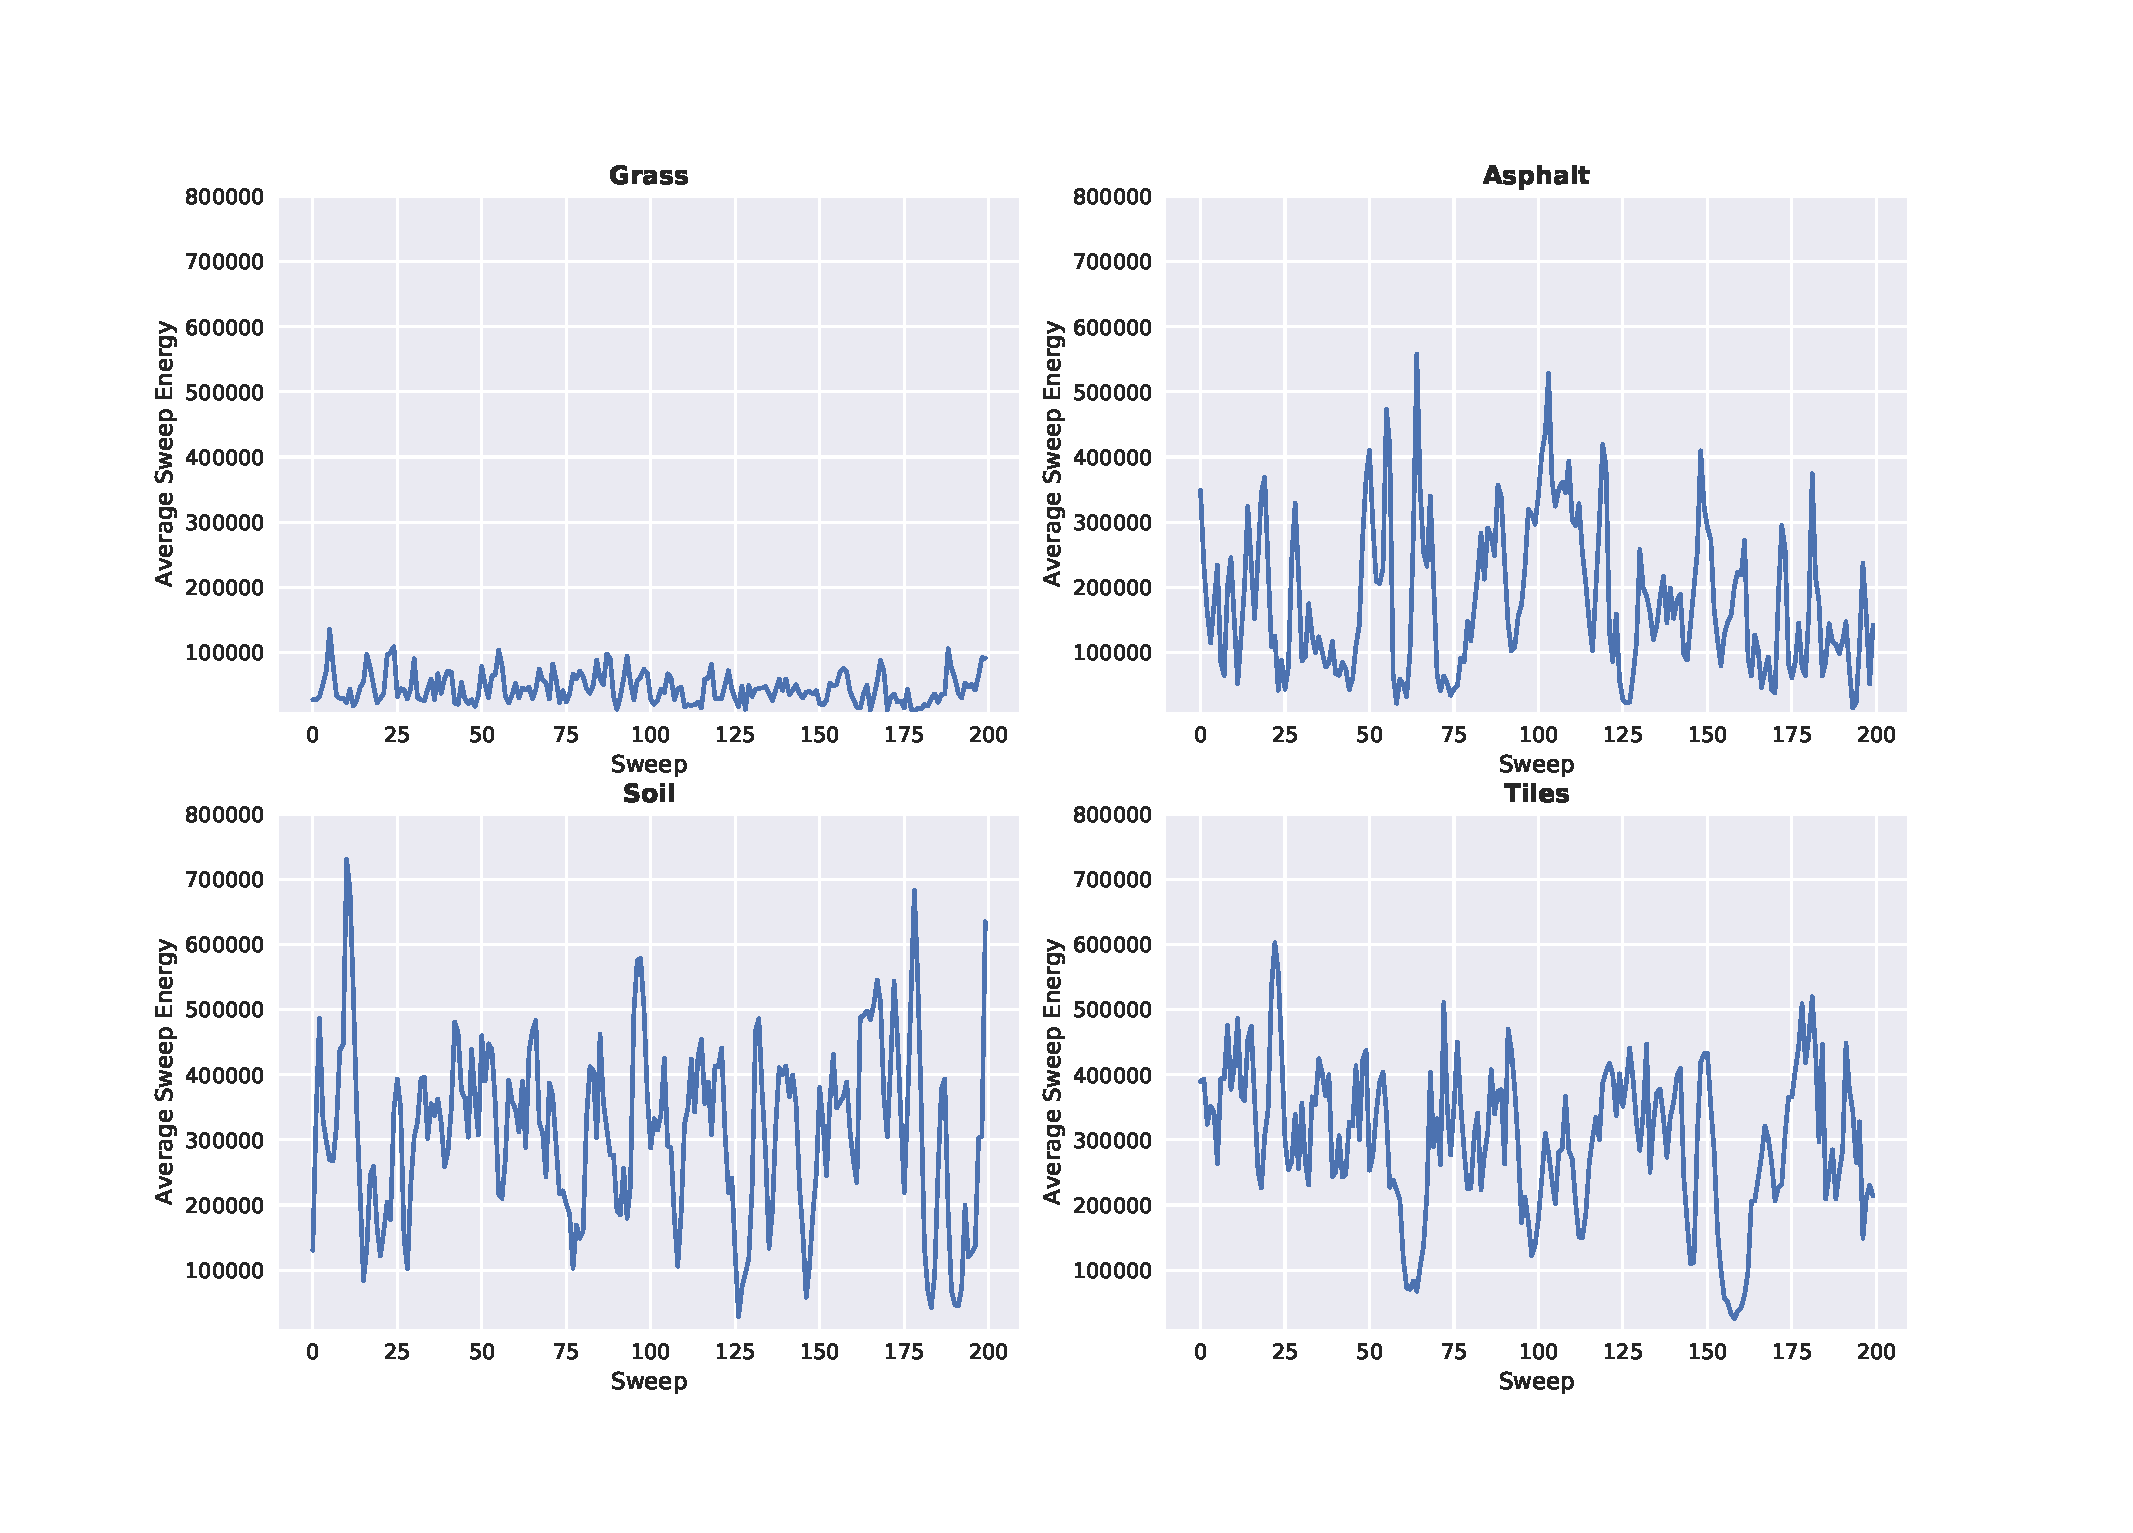
\includegraphics[scale=0.45]{figs_temp/features/sweep_energy}
	\caption{The figure shows the average sweep energy for 200 sweeps and four different materials. All measurements were made during a short period of time. The reflections from the grass surface carry noticeably less energy than those from the other surfaces. }
	\label{fig:sweep_energy}
\end{figure}



\subsection{Fourier Transform}
The surface underneath the radar can be assumed to be static, whereas the radar traverses the surface at a constant speed. This causes the radar to detect doppler frequencies. Depending on the surface's characteristics, the doppler frequencies may vary, (according to figure *Figure comparing reflections on a flat and rough terrain*?) and to visualize the frequency contents of different measured materials, the discrete Fourier transform is used. 

To compute the Fourier transform, a "box" consisting of $T$ sweeps is selected. Viewing this as a matrix with elements $X_{n,t}$, where $n$ denotes slow time, and $t$ fast time we can write a Fourier transform in slow time at range $r$, within this box as
\begin{equation}
	\mathbb{X}_k^{(r)} = \sum_{n=0}^{T-1}X_{n,r}\exp\Big[-2\pi i\frac{nk}{T}\Big] \quad k=0, ..., T-1.
\end{equation}
In figure \ref{fig:fft} five consecutive 128-step Fourier transforms have been computed for four materials. For grass (top plot), it can be seen that the frequency content is contained mainly at the start of the "FFT blocks", which corresponds to normalized frequency 0. The other materials contain slightly higher frequency content as well.

To avoid aliasing we refer to chapter earlier in report where this is discussed. Mention that $\mathbb{X}_k^{(r)}$, for all $r$, $k$, is flattened to a vector, resulting in one new sample.

\begin{figure}[h]
	\centering
	\includegraphics[scale=0.4]{figs_temp/features/fft}
	\caption{Each plot shows 5 concatenated DFTs, which have all been estimated from 128 consecutive sweeps. This has been done for ranges 7-23 cm, and the materials included in the figure are grass, asphalt, soil and tiles, respectively. Each FFT box has an $x$-axis going from normalized frequency 0 to 1.}
	\label{fig:fft}
\end{figure}




\subsection{Variance}

Assume $x(n,t)$ are samples from a complex normal distribution $X_{n,t}$. Variance $v_i(t_m)$ at range $i$ at time $t_m$ can then be approximated using

\begin{equation}
\label{eq:var}
\begin{gathered}
	v_i(t_m) = \E\{ (X_{i,t_m} - \E\{X_{i,t_m}\})^2\} \\
	= \frac{1}{T-1}\sum_{t=0}^{T-1}(x(i, t_m + t) - s_i(t_m))^*(x(i, t_m + t) -  s_i(t_m))
\end{gathered}
\end{equation}

\subsection{Autocovariance in slow time}

\textbf{Add some motivation for using autocovariance}

\noindent
For some stochastic process $P_t$ we can define the autocovariance $\gamma$ as

\begin{equation}
	\gamma(t, s) = \E\big\{(P_t - \mu_t)(P_s - \mu_s)\big\}
\end{equation}

If $X_t$ is a weakly stationary process the first moment (mean) and autocovariance do not vary over time.  The autocovariance then only depends on the difference between $s$ and $t$, making it possible to rewrite as

\begin{equation}
	\gamma(\tau) = \E\big\{(P_t - \mu)(P_{t+\tau} - \mu)\big\}
\end{equation}

Assuming weak stationarity over a few rangebins we can estimate the autocovariance in slow time for each selected range. 

\begin{equation}
\begin{gathered}
	\gamma_i(t_m, \tau) = \E\big\{(X_{i,t_m} - \E\{X_{i, t_m}\})^*(X_{i, t_m+\tau} - \E\{X_{i, t_m+\tau}\})\big\}\\
	= \frac{1}{T-1}\sum_{t=0}^{T-1-\tau}(x(i, t_m + t) - s_i(t_m))^*(x(i, t_m + t + \tau) - s_i(t_m + \tau))
\end{gathered}
\end{equation}•

We can drop the $\tau$ in the final expectation term, as $s_i(t)$ are estimated in batch from $t_m$ to  $t_m + T$ yielding

\begin{equation}
	\gamma_i(t_m, \tau) = \frac{1}{T-1}\sum_{t=0}^{T-1- \tau}(x(i, t_m + t) - s_i(t_m))^*(x(i, t_m + t + \tau) - s_i(t_m))
\end{equation}
as our expression for autocovariance. Note that the variance in \ref{eq:var} collapses to the autocovariance at 0 lag. 


\rowcolors{2}{gray!25}{white}
\begin{table}
\begin{center}
  \begin{tabular}{|c|cccc|}
\hline
    \rowcolor{blue!35}
                  & Abs & AC Energy & AC Range & FFT\\
    Config 1 & X & & & \\
    Config 2 &  & X & X&\\
    Config 3 & & & &X\\
    Config 4 & & & &\\
\hline
  \end{tabular}
\end{center}
\caption{Feature configurations}
\end{table}

\section{Mutual information}

In (link to information section) it was briefly discussed that information theory metrics can be utilized when considering which data is of interest. 

While a useful metric, estimating MI can be a non-trivial task. k-nearest neighbors introduced here:
\citep{kraskov_stögbauer_grassberger_2004}

The particular link between continuous features and discrete values that we use are itnroduced  here:
\citep{ross_2014}
